\section{Introducción} \label{introduccion}
\AddToShipoutPictureBG*{
\includegraphics[width=\paperwidth,height=\paperheight]{Imagenes/Fondo Capitulo 1.pdf}}
\thispagestyle{plain}

\divider

Previo a comenzar con el diseño de la placa de circuito impreso, debemos introducir la plataforma que se tiene que plasmar en esta PCB, explicando brevemente su funcionamiento y los bloques principales y auxiliares que la componen. Se puede apreciar un diagrama de esta plataforma, separada en sus distintos bloques funcionales en la figura \ref{fig:plataforma}.\\

\begin{figure}[h]
    \centering
    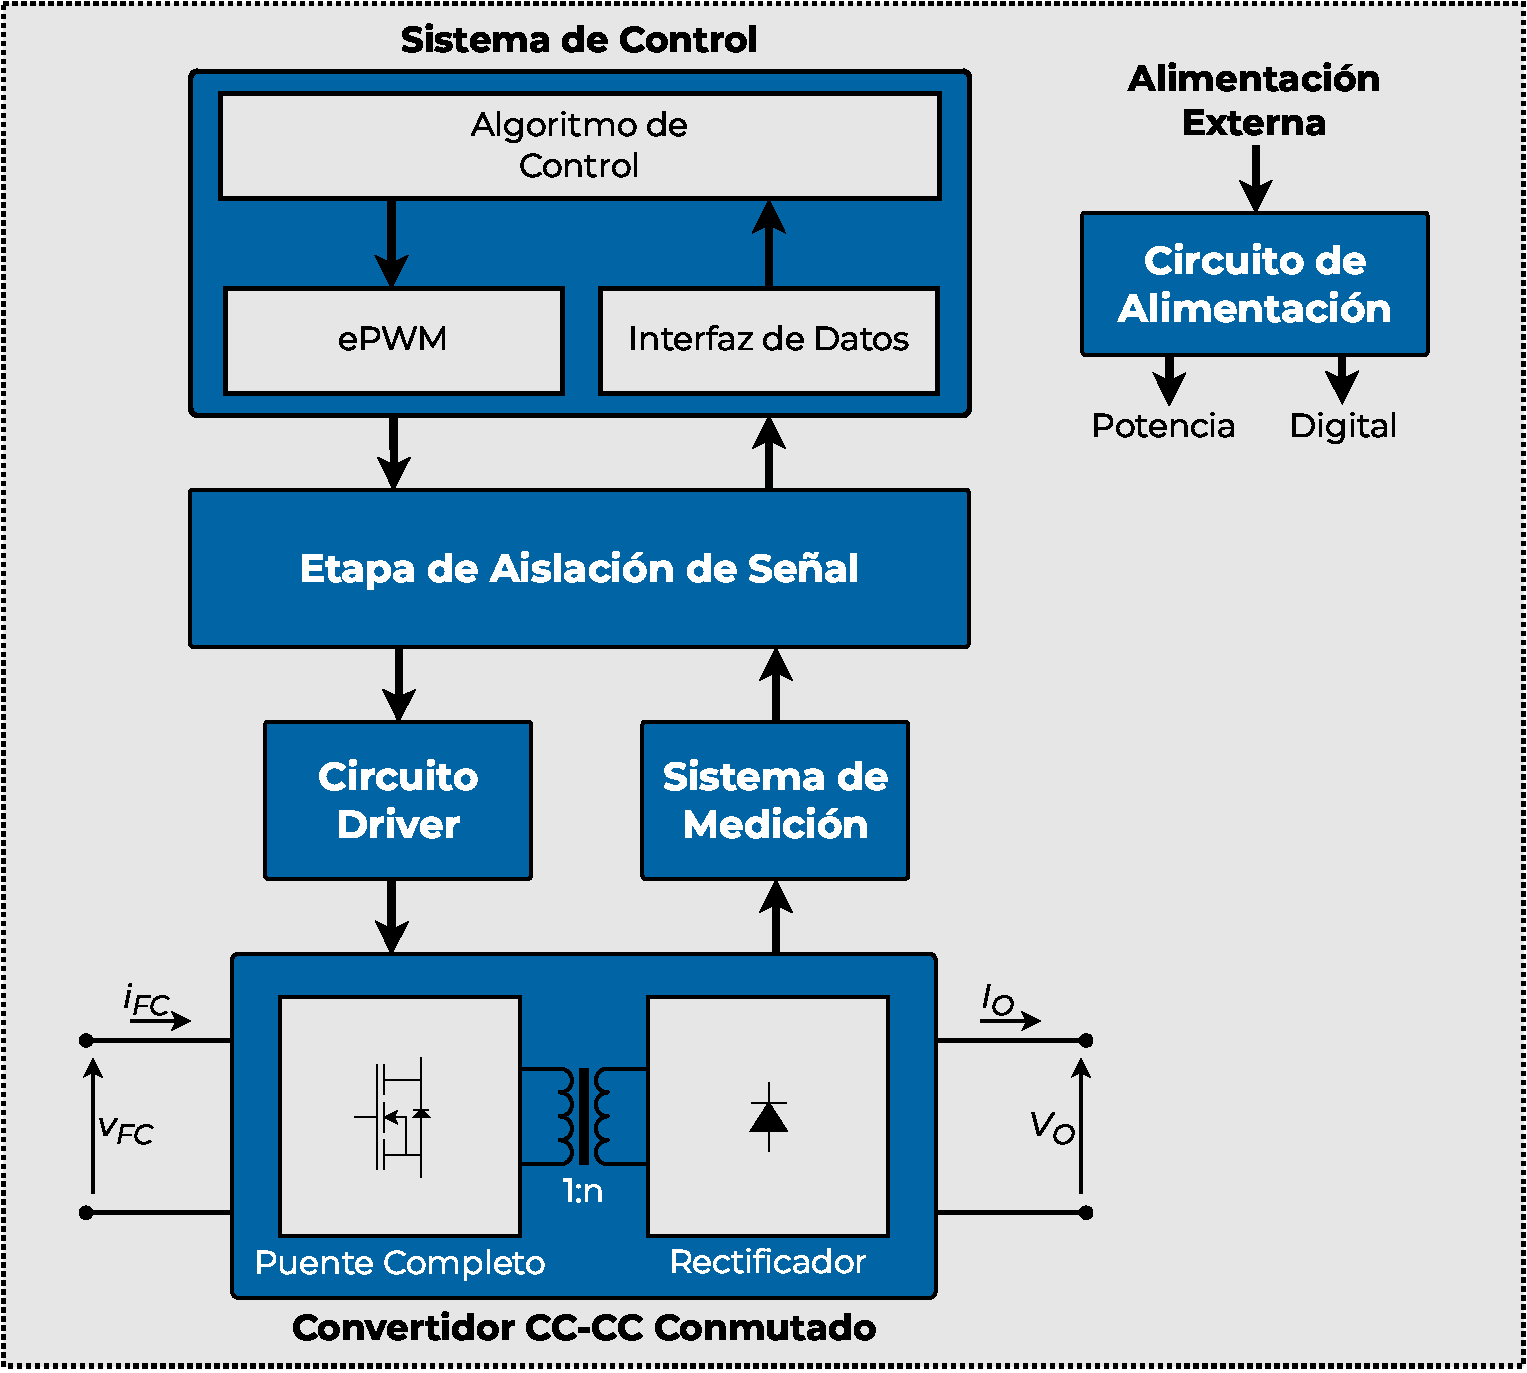
\includegraphics[scale=0.4]{Imagenes/Plataforma Detallada.pdf}
    \caption{Diagrama de la plataforma experimental de evaluación de celdas de combustible.}
    \label{fig:plataforma}
\end{figure}

Esta plataforma tiene como objetivo la adaptación de la interconexión de bloques en sistemas híbridos, sistemas complejos que combinan (o hibridan) múltiples módulos de generación y almacenamiento de energía, generalmente renovables, que luego se conectan a un bus de potencia de corriente continua (CC).\\

Particularmente, este sistema adapta el módulo de generación a partir de pilas de combustible para utilizar en un sistema híbrido, con una tensión de pila en la entrada $v_{FC}$ variable entre \SI[]{30}[]{\volt} y \SI[]{65}[]{\volt}, y una tensión de salida común fija de \SI[]{75}[]{\volt}. Para realizar esta la adaptación de estos niveles de tensión, se utilizó un convertidor CC-CC conmutado y aislado de tipo puente completo, que se regula mediante un sistema de control basado en un microcontrolador de tiempo real de la línea C2000 de Texas Instruments.\\

Previo a la realización de esta PPS, se trató el diseño circuital de la plataforma, construyendo los circuitos correspondientes a cada uno de los bloques que se muestran en la figura \ref{fig:plataforma}. Con estos circuitos diseñados, nos es posible pasar a su implementación en la placa de circuito impreso.\\